\begin{itemize}

\item \textbf{Papers and conference notes:}

    \begin{itemize}
        \item Conference note of~Beyond-the-Standard-Model light bosons search in Higgs decay to $4\ell$ channel at 13 TeV,  ATLAS-CONF-2017-042, Reference~\cite{ATLAS-CONF-2017-042}
    \end{itemize}
%%%%%%%%%%%%%%%%%%%%%%%%%%%%%%%%%%%%%%%%%%%%%%%%
%\item \textbf{Conference talks (APS, DPF, Physics Workshop, International Conferences):}
%
%    \begin{itemize}
%    \end{itemize}

%%%%%%%%%%%%%%%%%%%%%%%%%%%%%%%%%%%%%%%%%%%%%%%%
\item \textbf{ATLAS talks (approval talks, ATLAS weekly, or open presentations):}

    \begin{itemize}
        \item 06/2017, Open presentation, Search for Higgs decays to beyond the standard model light bosons in four-lepton events with the ATLAS detector $\sqrt{s}=$ 13 TeV, \url{https://indico.cern.ch/event/645640/}
    \end{itemize}
%%%%%%%%%%%%%%%%%%%%%%%%%%%%%%%%%%%%%%%%%%%%%%%%
%\item \textbf{Leadership roles (convenership, contact person, contact editor):}
%
%    \begin{itemize}
%        \item 04/2015-04/2016, ATLAS Standard Model Electroweak Group co-convener
%        \item 04/2016-04/2017, ATLAS XYZ Team co-contact
%        \item ...
%    \end{itemize}
%%%%%%%%%%%%%%%%%%%%%%%%%%%%%%%%%%%%%%%%%%%%%%%%
\item \textbf{Hardware, software, performance and other service work contributions:}

        \begin{itemize}
       	 \item Hardware contribution: I contributed to installing and commissioning of 12 BMG chambers during 2017 winter shut down. I am also studying space charge effect in MDT chambers by looking at readout charge gain and spatial resolution.
        \end{itemize}
%%%%%%%%%%%%%%%%%%%%%%%%%%%%%%%%%%%%%%%%%%%%%%%%
\item \textbf{Analysis Contributions:}

        \begin{itemize}
       	 \item For Conf Note 1, I contributed to $H \rightarrow XX \rightarrow 4\ell$ High mass part in: Z Veto cut optimization, cross check of cutflow, cross check of systematic variation and upper limit setting using toy Monte Carlo (Figure ~\ref{fig:Rongkun_ZdZd_Limit}).
        \end{itemize}
        
        \begin{itemize}
       	 \item I am making major contributions to inclusive m4l unfolding analysis, including unfolding method study, optimization of binning and statistical tests using Bayesian reasoning.
        \end{itemize}
        
        \begin{itemize}
       	 \item I contributed in HZZ group for several analyses in evaluating qqZZ theory uncertainties, including showering, scale and pdf systematics.
        \end{itemize}
	 
        \begin{figure}[!htbp]
        \begin{center}
            \subfloat[Fiducial cross sections\label{fig:Rongkun_ZdZd_Limit_fid}]{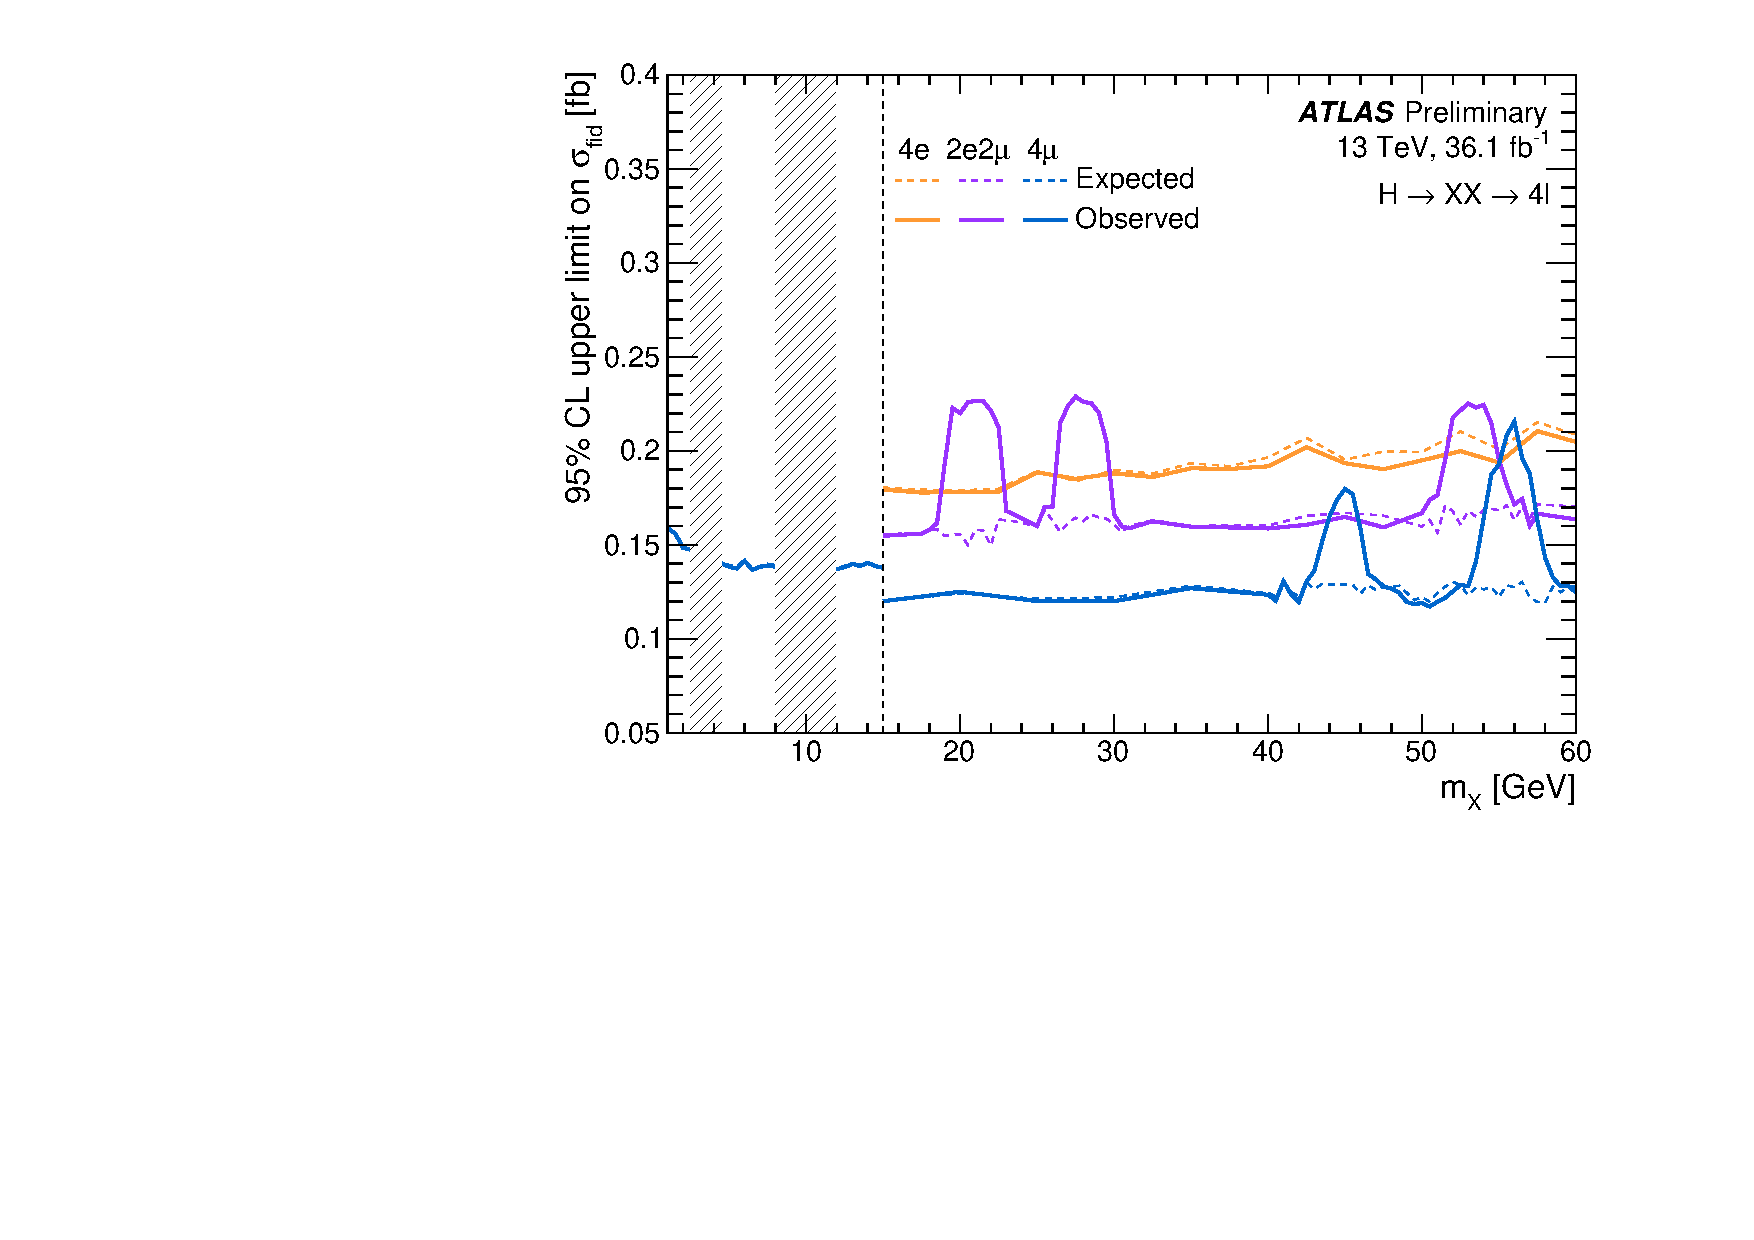
\includegraphics[width=0.49\textwidth]{../figures/Rongkun-ZdZd_limit_fid.pdf}}
            \subfloat[Branching Ratios\label{fig:Rongkun_ZdZd_Limit_tot}]{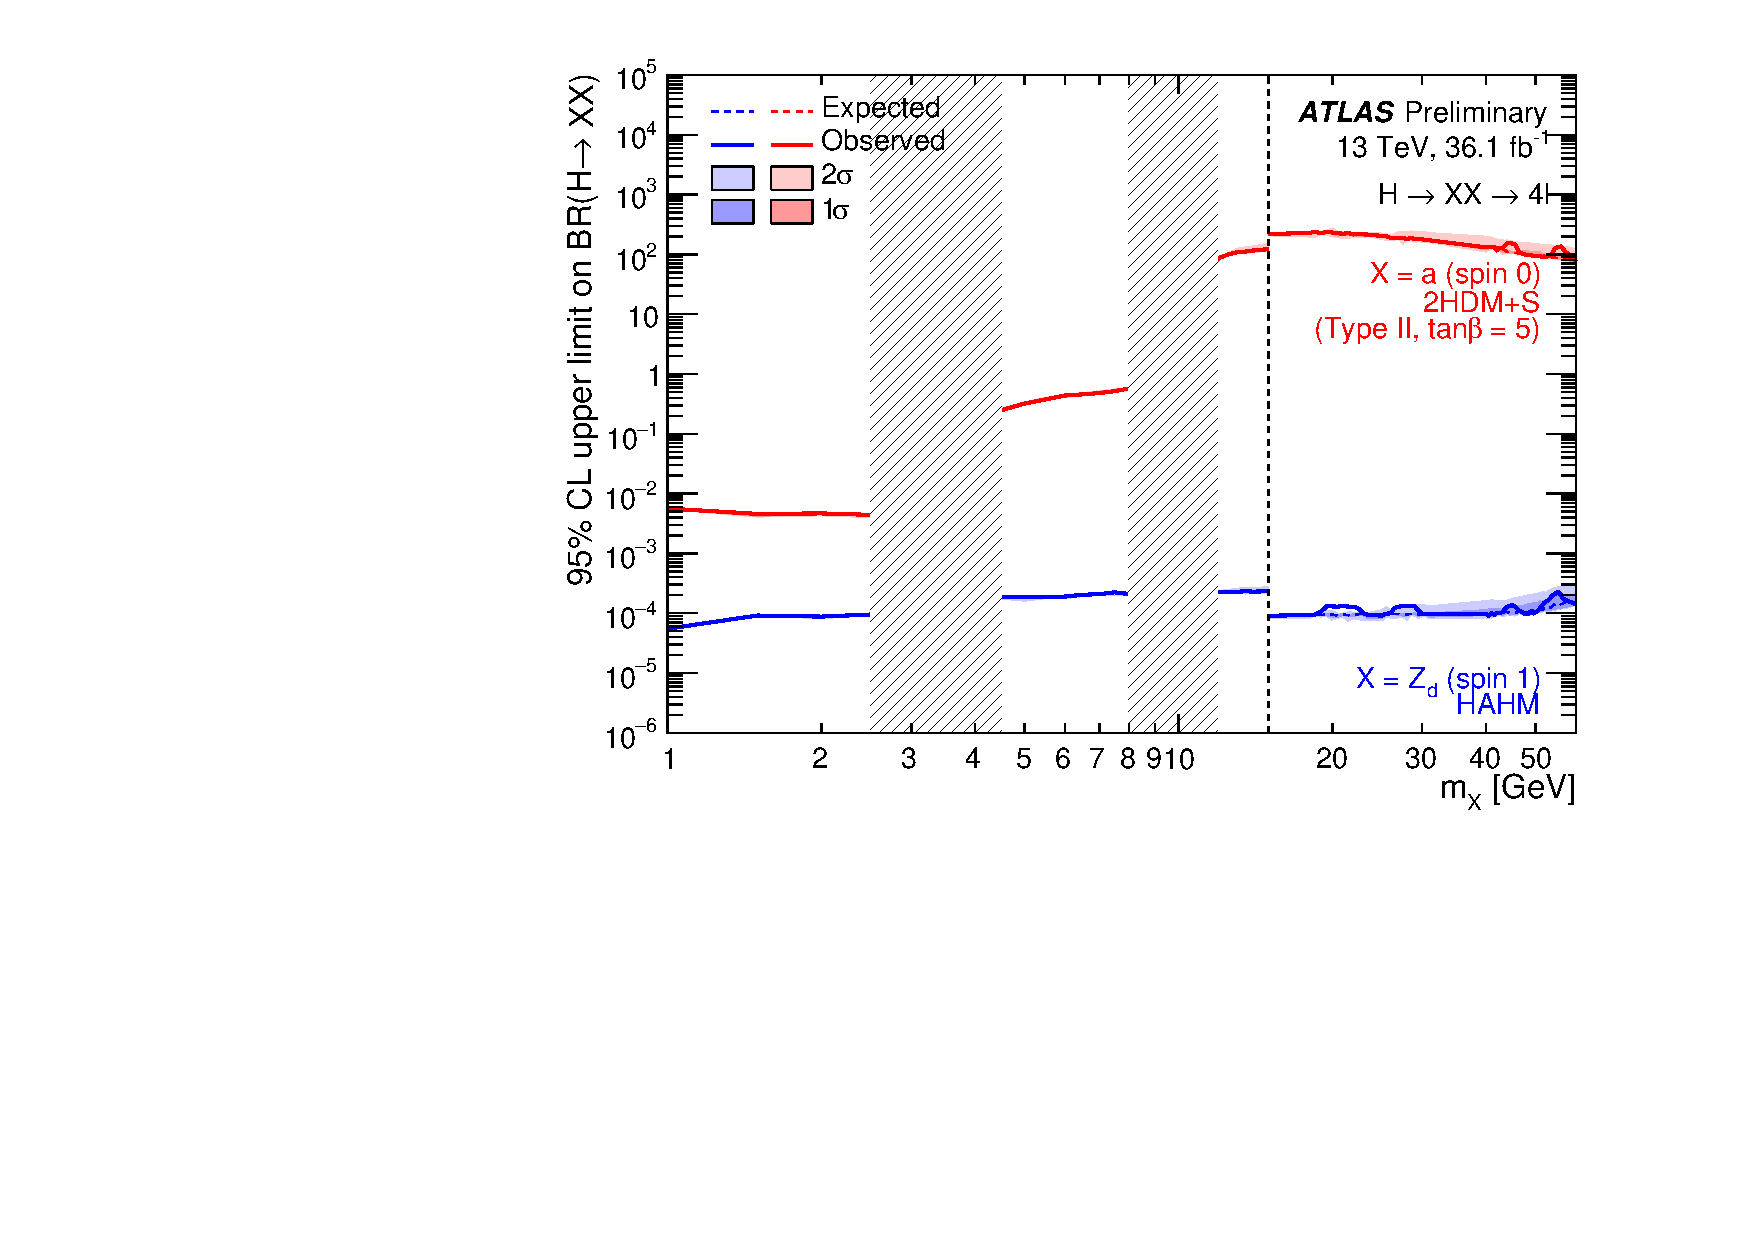
\includegraphics[width=0.49 \textwidth]{../figures/Rongkun-ZdZd_limit_tot.pdf}}
            \caption{95\% CL upper limits of the process $H \rightarrow XX \rightarrow 4\ell$ on (a) model-independent fiducial cross sections, and (b) branching fractions BR($H\rightarrow Z_{d}Z_{d}$) and BR($H\rightarrow aa$) for the two benchmark models considered.}
                \label{fig:Rongkun_ZdZd_Limit}
        \end{center}
        \end{figure}

\end{itemize}
